%------------------------------------------------------------------------------
% Template file for the submission of papers to IUCr journals in LaTeX2e
% using the iucr document class
% Copyright 1999-2003 International Union of Crystallography
% Version 1.2 (11 December 2002)
%------------------------------------------------------------------------------
%
\documentclass[preprint]{iucr}              % DO NOT DELETE THIS LINE
                   \def\href#1{\relax}\let\foo\caption
\ifPDF
  \RequirePackage{hyperref}
  \PassOptionsToPackage{pdftex,bookmarksopen,bookmarksnumbered}{hyperref}
  \voffset=-0.5in
\fi
\let\caption\foo

\usepackage{graphicx}
\usepackage[T1]{fontenc}
\usepackage[utf8]{inputenc}
 \usepackage{amsmath}
%\usepackage{eps2pdf}

 \paperprodcode{a000000}      % Replace with production code if known
 \paperref{gy5006}            % Replace xx9999 with reference code if known
 \papertype{IU}               % Indicate type of article
 \paperlang{english}          % Can be english, french, german or russian
 \journalcode{S}              % Indicate the journal to which submitted
 \journalyr{2019}
 \journalreceived{\relax}
 \journalaccepted{\relax}
 \journalonline{\relax}

\begin{document}                  % DO NOT DELETE THIS LINE

\title{New tools for calibrating diffraction setups}
\shorttitle{Calibration tools in pyFAI}
 
 \cauthor[a]{J.}{Kieffer}{jerome.kieffer@esrf.eu}

 \author[a]{V.}{Valls}
 \author[b,c]{N.}{Blanc}
 \author[d,e]{C.}{Hennig}
 
 \aff[a]{ESRF, The European Synchrotron, CS40220, 38043 \city{Grenoble}
 Cedex 9, \country{France}}
 \aff[b]{University Grenoble Alpes, Grenoble INP,  38000 \city{Grenoble}, \country{France}}
 \aff[c]{CNRS, Institut NEEL, 38000 \city{Grenoble}, \country{France}}
 \aff[d]{Helmholtz-Zentrum Dresden-Rossendorf, Institute of Resource Ecology, 
Bautzner Landstrasse 400, 01328 \city{Dresden}, \country{Germany}}
 \aff[e]{The Rossendorf Beamline at ESRF, BP 220, 38043 \city{Grenoble}
 Cedex 9, \country{France}}
 \shortauthor{Kieffer & al.}


\keyword{Powder diffraction}
\keyword{translation table}
\keyword{goniometer}
\keyword{geometry calibration}
\keyword{pair distribution function}



\maketitle                        % DO NOT DELETE THIS LINE

\begin{synopsis}
New tools to calibrate different types of scattering experiments suitable for static
and moving detectors.
\end{synopsis}

\begin{abstract}


This work presents new calibration tools in the pyFAI
suite for processing scattering experiments acquired with area detectors:
a new graphical user interface for calibrating the detector position in a  
scattering experiment performed with a fixed, large area detector as well as 
a library to be used in \textit{Jupyter notebooks} for calibrating the motion
of a detector on a goniometer arm (or any other moving table) to perform
diffraction experiments.
\end{abstract}


\section{Introduction}

According to an internal survey performed among the beam-line scientists at
the European Synchrotron (ESRF) in 2016, the factor limiting the users'
productivity at diffraction beam-lines is the calibration of the experimental
setup before accessing to the raw data for their reduction. 
The calibration issue is currently worked around by providing users with the
proper geometry description or even the reduced data, but this prevents the
re-processing at home institutes and also the re-interpretation of data which
is needed as a part of the open data initiative.

At X-ray facilities like synchrotons, large area detectors are 
preferred for gathering a maximum number of photons in
scattering experiments (powder diffraction, small angle
scattering, \ldots).
% The still position of the detector during the acquisition, makes also
%easier the data-reduction step.
Using a fixed position setup combined with the speed of modern detectors (up
to a few kHz) the data acquisition \textit{in situ} is easily
performed to follow chemical reactions or other physical processes.
Even with fixed geometries, determining the detector's position is
still an issue for a majority of users. 
Hence, a new graphical user interface has been developed for pyFAI
\cite{pyFAI_0.18}, focusing on the user's experience to grant them autonomy in
data analysis, once they are back in their home institutes.

Unlike synchrotron sources, laboratory source diffractometers
are commonly equipped with (small) area detectors mounted on moveable goniometer
arms for powder diffraction (for example, the Rigaku HyPix-3000 detector),
%The larger number of pixels trades-of the resolution for speed.
whereas detectors at synchrotrons are often mounted on goniometer or
translation tables, those degrees of freedom (hereafter $dof$) are rarely used for data
acquisition.
One counter-example is reported in \cite{Gao:kc5032}, where the beam-line
is equipped with a moving strip-detector, the Mythen detector (1D) from Dectris,
which is not an area detector.

%On the opposite, moving detector setups are rarely
%used at synchrotrons for the data acquisition itself, even if most of the
% detectors are mounted on a moving table or on a goniometer. 



%High-Q diffraction signal acquisition is needed  for
Pair Distribution Function (\textsc{pdf}) analysis requires very large
detectors and higher energies to be able to cover the needed high $q$-range in
one single frame \cite{Chupas:wf5000}.
When speed is not critical, \textsc{pdf} experiments could be performed
with smaller detectors mounted on a motorized arm, and moved in front of
the sample during the data acquisition to cover a larger solid angle. 
This kind of setup is actually already available on most diffraction
beam-lines. 
A new pyFAI module dealing with goniometers and moving detectors is also presented.

The pyFAI library \cite{fv5028}, is briefly introduced, followed by a description of
how to merge multiple diffraction images acquired at different positions with this
library \cite{PyFAI_PDJ}. 
After summarizing how calibration works in pyFAI, the new graphical user
interface is presented.
Finally, the procedure on how to calibrate the absolute position of
every single pixel in the detector when mounted on a goniometer (or on a
translation table) as a function of the goniometer motor positions, is
described assuming actuators are precise and coupled with encoders. 

\section{The Python Fast Azimuthal Integration library (pyFAI)}

PyFAI is a Python \cite{python} library used to transform 2D diffraction images into
1D powder diffraction patterns by re-binning the pixel positions in polar
coordinates. 
The radial units are typically the scattering angle  
$2\theta$ or the momentum transfer $q=4\pi \sin(\theta)/\lambda$.
PyFAI also provides tools to calibrate the detector position, i.e.
to determine its location in space by means of Debye-Scherrer conical rings
resulting from the intersection of the diffracted X-ray beam with the
detector surface. 
The rings are deformed into ellipses when the detector is planar but 
slightly inclined. 
The azimuthal integration is performed in two steps. 
The first is a pixel-wise
transformation corresponding to the image correction:

\begin{equation}
I_{cor} = \frac{signal}{normalization}  = \frac{I_{raw} - I_{dark}}{F \cdot
\Omega \cdot P \cdot A \cdot I_0} 
\end{equation}

where $I_{raw}$ is the detector's raw signal, $I_{dark}$ is the dark current
image (it may also be the background image for certain experiments), $F$ is a 
factor accounting for the flat-field correction, $\Omega$ is the solid
angle subtended by a given pixel, $P$ is the polarisation correction term and
$A$ represents the detector's apparent efficiency due to the incidence angle of the
photon on the detector (for integrating detectors, high energy photons with
larger incidence angle see larger sensor thickness, and thus have higher
detection probability).
$I_{raw}$ may be normalized by the incoming flux $I_0$, which is
independent of the pixel position.
The numerator of equation (1) will hereafter be referred as
\textit{signal}, whilst the denominator will be referred as
\textit{normalization}. 
The \textit{variance} associated to the \textit{signal} of every single pixel can be estimated 
from statistical distributions assuming for example the detecor has a Poissonian behaviour. 
This \textit{variance} needs to be scaled in a similar way when considering error propagation.

The second step is the re-binning of the data, which is carried out 
using a histogram of the $q$ or $2\theta$ values, weighted by the
\textit{signal}.
This gives the sum of all \textit{signals} within a Debye-Scherrer ring.
A second ($q-$ or $2\theta-$) histogram is calculated, weighted
by the \textit{normalization} this time, which gives the sum of all
normalised factors falling into the given bin.

The average signal over a ring is then simply the ratio of two histograms (2) 
while its associated error, the standard error of the mean, is given by (3):

\begin{equation}
\overline{I_{ring}} = \frac{\sum\limits_{i \in ring} c_i \cdot signal_i}
                        {\sum\limits_{i \in ring} c_i \cdot normalization_i} 
\end{equation}
\begin{equation}
\sigma(I_{ring}) = \frac{\sqrt{\sum\limits_{i \in ring} c_i^2 \cdot variance_i}}
                  {\sum\limits_{i \in ring} c_i \cdot normalization_i} 
\end{equation}

In equations (2) and (3), $c_i \in [0..1]$ corresponds to the fraction of a pixel area 
falling into a specific histogram bin. 
PyFAI provides multiple pixel splitting schemes that differ only by their
respective $c_i$ coefficients. 
Simple un-weighted histograms correspond to deactivate pixel splitting; in this
case $c_i$ is one only for pixels falling in the corresponding bin an zero for all
the others.

This is an improvement over former versions of pyFAI where pixels with
smaller area, further away from the sample or weaker were overrepresented in
the statistic :
\begin{equation}
\overline{I_{ring}} = \frac{\sum\limits_{i \in ring} \frac{ c_i \cdot
signal_i}{normalization_i}} {\sum\limits_{i \in ring} c_i} 
\end{equation}

The multiple pixel splitting schemes available in pyFAI, called full-splitting, 
bounding-box-splitting and no-splitting, have already been described in
 \citeasnoun{fv5028} and can be stored as sparse matrices to accelerate the
 calculation of the histograms \cite{kieffer_ashiotis-proc-euroscipy-2014}.

\section{Azimuthal integration of multiple frames taken at multiple geometries}

The pyFAI integration scheme of multiple images taken at varying positions has
first been reported in  \cite{PyFAI_PDJ}. 
The procedure is conceptually similar to the integration on a single image,
except that the various histograms, all calculated over the same
grid, are summed together, i.e. \textit{signals} and, separately, 
\textit{normalizations} from all images as follows: 

\begin{equation}
\overline{I_{ring}} = \frac{\sum\limits_{imges} \sum\limits_{i \in ring} c_i \cdot
signal_i} {\sum\limits_{imges} \sum\limits_{i \in ring} c_i \cdot
normalization_i} 
\end{equation}

The normalization for solid angle correction $\Omega$ has to be performed
using an absolute solid angle reference system (unlike the case of single
frame integration) as different geometries may have very different
sample-to-detector distances.
Hence single image integrated intensity in multi-geometry mode is orders of
magnitude larger than using the ``normal'' pyFAI integration methods.

\section{Calibration of the detector position}

\subsection{Principle of the calibration using a Debye-Scherrer diffraction
image}
The calibration of a detector position is performed using a few Debye-Scherrer
rings (minimum 2) collected from a reference powder called \textit{calibrant}.
The rings are extracted automatically and control points are placed at the
local maxima on the rings.
The geometry of the experiment is obtained from least-squares fitting of
the $2\theta$ values calculated for the different control points.
%In this work we will call them ``rings'' even if, for planar detector,
%they are actually the conic intersections of the X-ray beam cones
%with the detector plane.
For non-planar detectors these ``rings'' can be any curve, while on planar 
detectors in transmission mode, they are simply ellipses.

Intuitively, the easiest geometry to perform the calibration is built upon 
the beam-center definition, this is the intersection of the direct beam with the detector. 
This geometry has been first introduced in FIT2D \cite{Hammersley:fs5107} 
and re-used in many software packages like GSAS-II \cite{Toby:aj5212} and 
Dawn \cite{Filik:vg5068} which offer more user-friendly interfaces.
The FIT2D-geometry reaches its limits when the detector is heavily tilted, and it is not 
even possible to describe a detector mounted parallel to the beam (which is sometimes used in 
reflection geometry).
PyFAI's geometry has been inspired by SPD \cite{Boesecke:aj6013} which is able to describe any 
detector position in space. 
This geometry is based on the concept of Point Of Normal Incidence 
(hereafter named \textsc{poni}, Figure \ref{poni}), which is 
the orthogonal projection of the sample position (origin) on the detector plane (or
the plane $z=d_3=0$ when the detector is non-planar and $z$ varies from pixel to pixel).
It is worth noting that the \textsc{poni} is co-located with the beam-center when the 
detector is not tilted but 
the \textsc{poni} is more likely than the beam-center to be located within the detector's 
surface when the detector is heavily tilted. 
Indeed, a detector facing the sample allows to gather a maximum amount of photons scattered.
Conversion tools between geometries are provided by pyFAI and documented in \cite{Detlefs2019}.

The least-squares refinement is optimizing a set of six geometrical parameters:
the three translations corresponding to the coordinates of the \textsc{poni} and
the three rotations corresponding on the tilt of the detector around three orthogonal axes.
This makes seven parameters to refine when considering in addition the energy or the wavelength. 


\begin{figure}
\label{poni}
\begin{center}
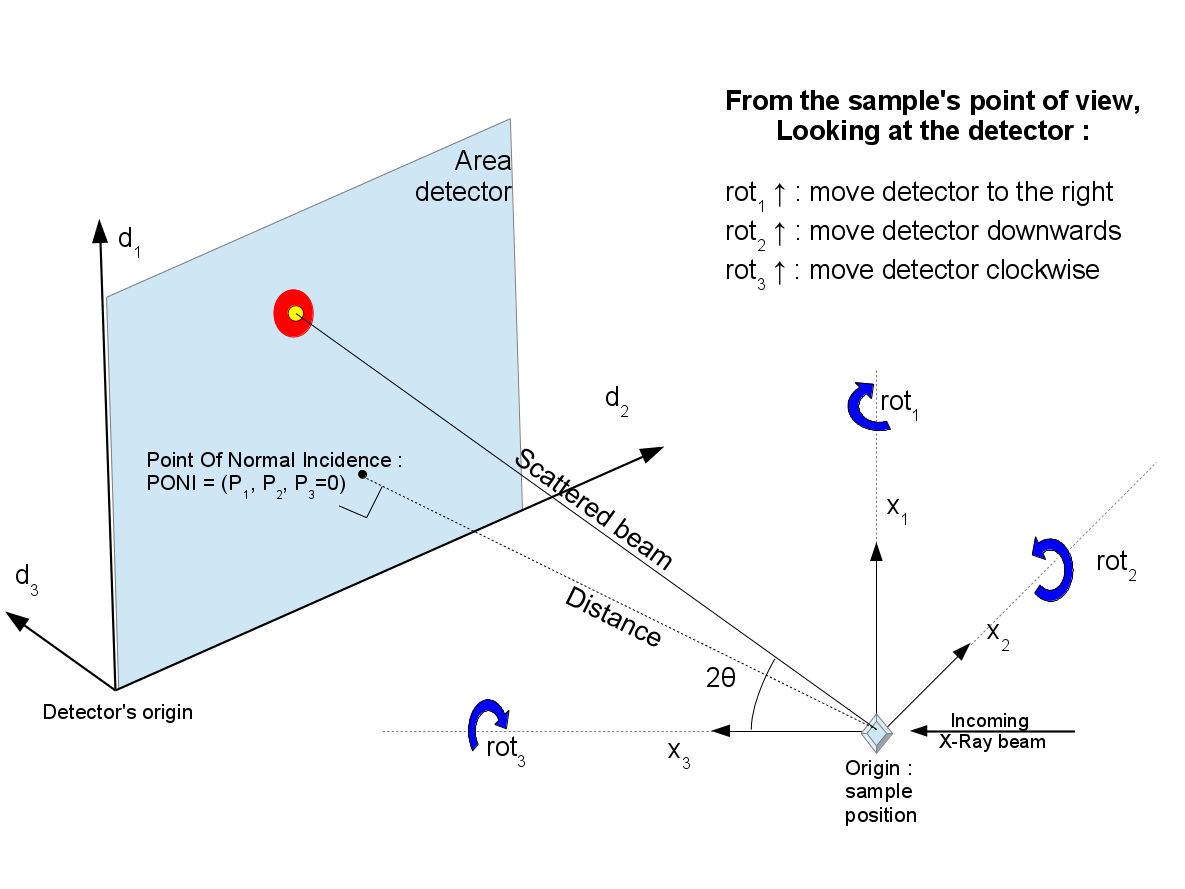
\includegraphics[width=15cm]{images/PONI}
\caption{Geometry used in pyFAI.}
\end{center}
\end{figure}


The parameters to be refined are the following:
\begin{itemize}
  \item $dist$: the distance (in metres) from the sample position to the
  \textsc{poni}.
  \item $poni_1$ and $poni_2$: space coordinates of the
  \textsc{poni} (in metres) within the detector plane ($z=d_3=0$) along the slow-
  and the fast-reading dimension of the detector image (1 and 2 usually refer to the row
  and the column axis, i.e. ``y, x'' respectively).
  \item $rot_1$, $rot_2$ and $rot_3$: the
  rotation angles (expressed in radians) of the detector placed at the proper
  distance from the sample, with respect to the 3 axes of the
  laboratory reference system.
  The detector is first rotated around the vertical axis ($rot_1$), then
  around the horizontal axis ($rot_2$) and in the end around the
  incoming beam direction ($rot_3$). In a more mathematical way, this gives:
\begin{equation}
	R = R_3 \cdot R_2 \cdot R_1 
\end{equation}
where
\begin{equation}
	R_1 = 	
	\begin{bmatrix}
	1 & 0 & 0\\
	0 & \cos(rot_1) & \sin(rot_1) \\
	0 & -\sin(rot_1) & \cos(rot_1) \\
	\end{bmatrix}
\end{equation}
\begin{equation} 		
	R_2 =
	\begin{bmatrix}
	\cos(rot_2) & 0 & \sin(rot_2) \\
	0 & 1 & 0 \\
	-\sin(rot_1)&0 & \cos(rot_2) \\
	\end{bmatrix}
\end{equation}
\begin{equation} 	
	R_3 =
	\begin{bmatrix}
	\cos(rot_3) & -\sin(rot_3) & 0 \\
	\sin(rot_3) & \cos(rot_3) & 0\\
	0 & 0 & 1\\
	\end{bmatrix}
	\cdot 
\end{equation}

It is worth mentioning rotations $R_1$ and $R_2$ are left-handed, while 
$R_3$ is right-handed. Changing this now would break the compatibility with
any former version of pyFAI.
\end{itemize}

The strength of this parameterization is that it describes any detector position in
space. 
The drawback is that some parameters are correlated or not optimized:

\begin{itemize}
  \item \textit{dist-wavelength}: reducing the wavelength is nearly equivalent
  to increasing the distance unless the diffraction angle $2\theta$ is actually
  large ($>30^o$). 
  It is advisable to fix one of the two variables unless the data are good
  quality and the scattering angles are large.
  \item $rot_1$-$poni_2$ and $rot_2$-$poni_1$, as small rotations can be
  mistaken for larger translations. 
  Fixing one of the two decreases the uncertainty of the other by a few orders of
  magnitude.
  \item $rot_3$ cannot be refined from Debye-Scherrer cones as they are, by definition,
  invariant by rotation around the incoming beam. The $rot_3$ parameter can be
   assessed using an anisotropic contribution, like the polarization effect or
  some  textures in the sample.
  This $rot_3$ parameter is also used to simulate the azimuthal rotation of
  the experimental setup or of the sample, for example when calculating pole
  figures.
\end{itemize}
 

The calibration parameters containing the geometry of the experimental setup are saved in a text file with the ``.poni''
extension, which contains in addition the detector definition and the wavelength.
This file can subsequently be loaded into an \textit{azimuthal integrator}
object, ready to perform the azimuthal integration.

\subsection{Graphical user interface}

A semi-graphical calibration tool has been available as part of pyFAI
\cite{fv5028} since the origin of the project, but this tool was considered too
difficult to use by inexperienced users.
Thus, many groups have developed their own graphical user interface on top of
pyFAI, often optimized for their specific setup or experiment.
For example: Dioptas \cite{diopta_publi} for high pressure, Dpdak \cite{dpdak}
for SAXS, NanoPeakCell \cite{nanopeakcell} for serial crystallography,
PySAXS \cite{pysaxs}, WiSAXS, xPDFsuite \cite{xpdfsuite}\ldots

Following the survey conducted among the beam-line scientists of the ESRF, a
new graphical user interface design was developed, based on the PyQt5
library \cite{pyqt} and specifically focusing on the needs of novice users, but
not on the type of experiment.
The calibration of the experimental setup based on Debye-Scherrer rings 
is carried out in five steps and presented as a software wizard with five
subsequent tabs within the graphical interface:
\begin{itemize}
  \item{Experimental settings:} This first tab lets the user select
  the wavelength (or the energy) used, the reference material used
  for calibration (called calibrant) and to choose the kind of detector among the
  list of 50 provided or to define a specific detector (Figure \ref{calib_1}),
  \item{Mask drawing:} This tab allows to mask-out unwanted regions/pixels from the
  image, either based on their intensity (thresholding) or simply by
  drawing polygons on the image. Different masks can be saved, retrieved and assembled (Figure \ref{calib_2}),
  \item{Peak picking:} Individual peaks and arc of rings can be segmented out
  (automatically) and assigned (manually) to different rings, each ring 
  being associated with a single reflection of the calibrant (Figure
  \ref{calib_3}),
  \item{Geometry fitting:} At this stage, the detector position and
  wavelength are fitted against peak positions and ring numbers. 
  Any of the  parameters can be fixed or let free for refinement.
  The (calculated) positions of the beam center and the \textsc{poni}
  and the expected positions of rings are overlaid to the diffraction image
  to assess visually the quality of the fit. Sample, detector 
  and direct beam can also be visualized in 3D (Figure \ref{calib_4}). 
  \item{Integration:} This tab displays the 1D and 2D integrated patterns, also
  called powder diffraction profile and caked-image to further validate the
  modelization of the experimental setup (Figure \ref{calib_5}). 
  The algorithm for integrating, the pixels splitting scheme and the radial unit
  can also be selected in this tab. 
  Diffraction profiles can be saved as text-files or images as well as the
  experimental setup description file (\textsc{poni}-file) for subsequent use with other tools from
  the pyFAI suite.
\end{itemize}

\begin{figure}
\label{calib_1}
\begin{center}
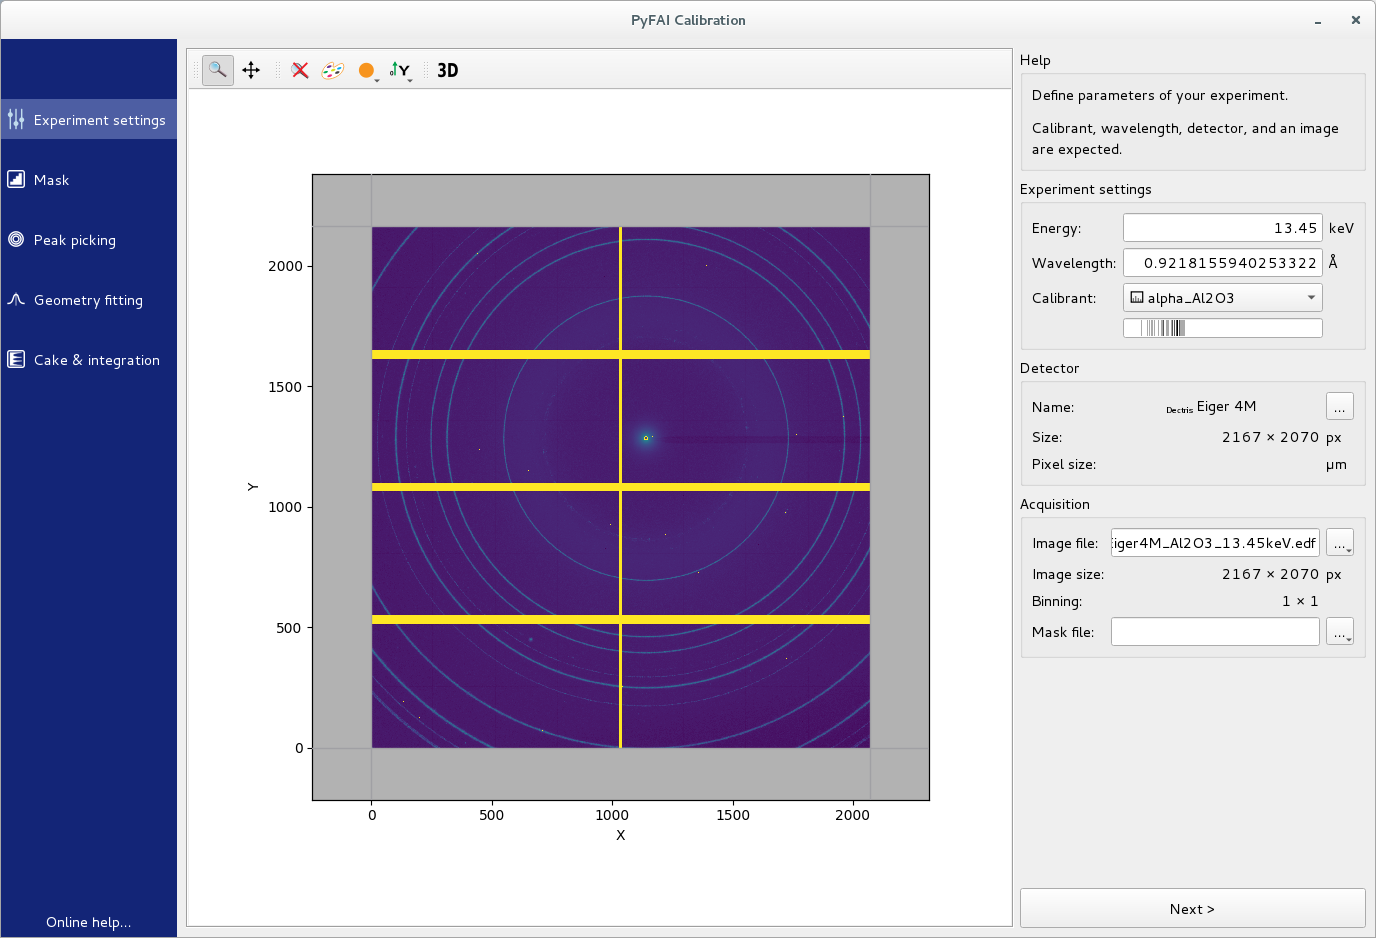
\includegraphics[width=15cm]{images/1_experiment}
\caption{Experiment settings tab: load the calibration image, set the energy, the calibrant and select the detector for the subsequent analysis.}
\end{center}
\end{figure}
\begin{figure}
\label{calib_2}
\begin{center}
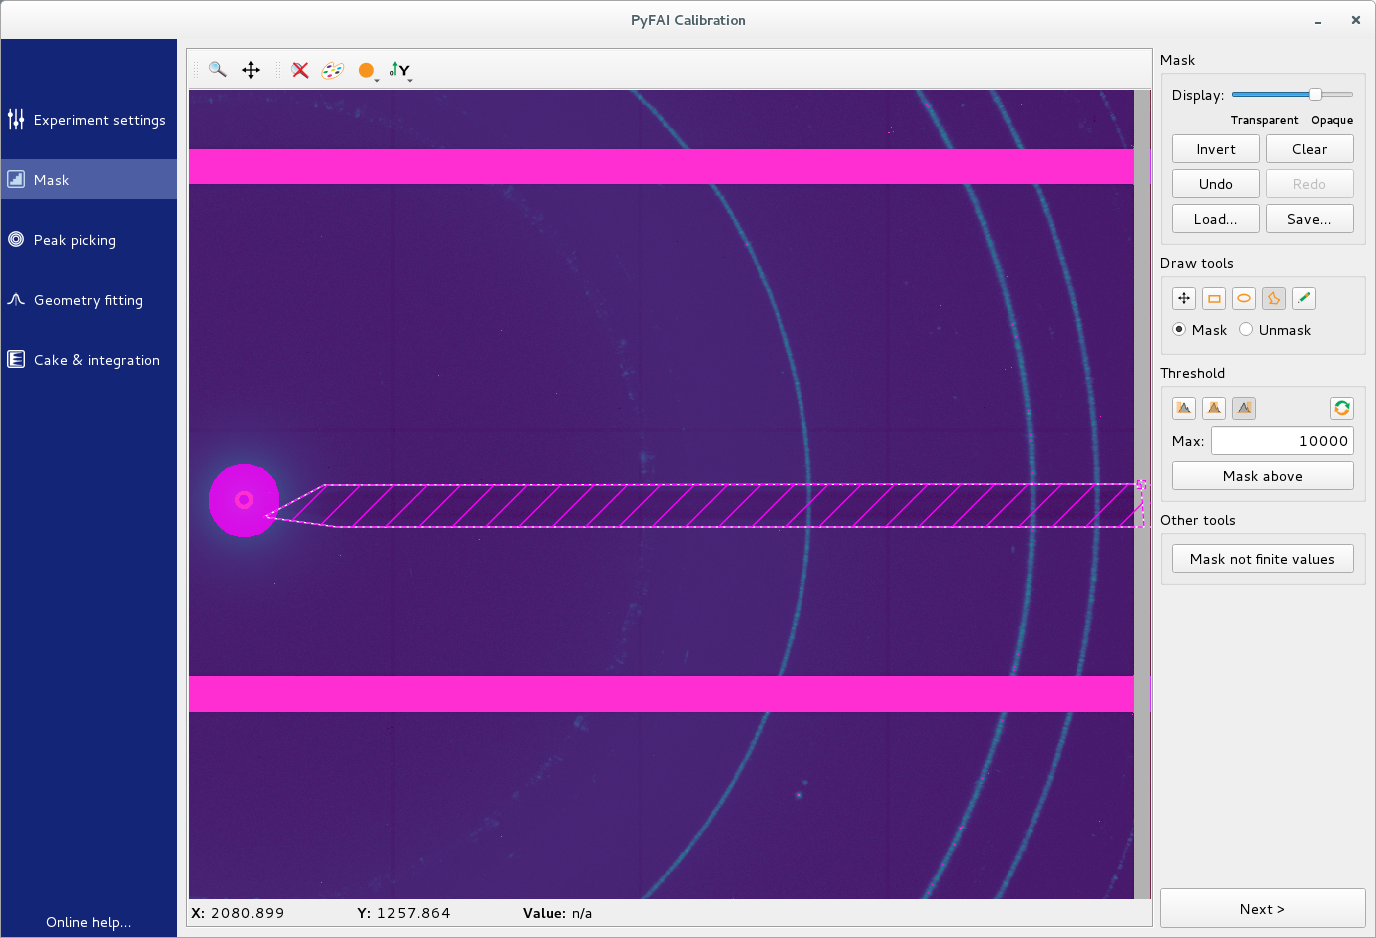
\includegraphics[width=15cm]{images/2_mask}
\caption{The mask drawing tool is used to exclude pixels using a rectangular, polygonal or pencil selection. 
         Pixels can also be selected according to their value (thresholding)}
\end{center}
\end{figure}
\begin{figure}
\label{calib_3}
\begin{center}
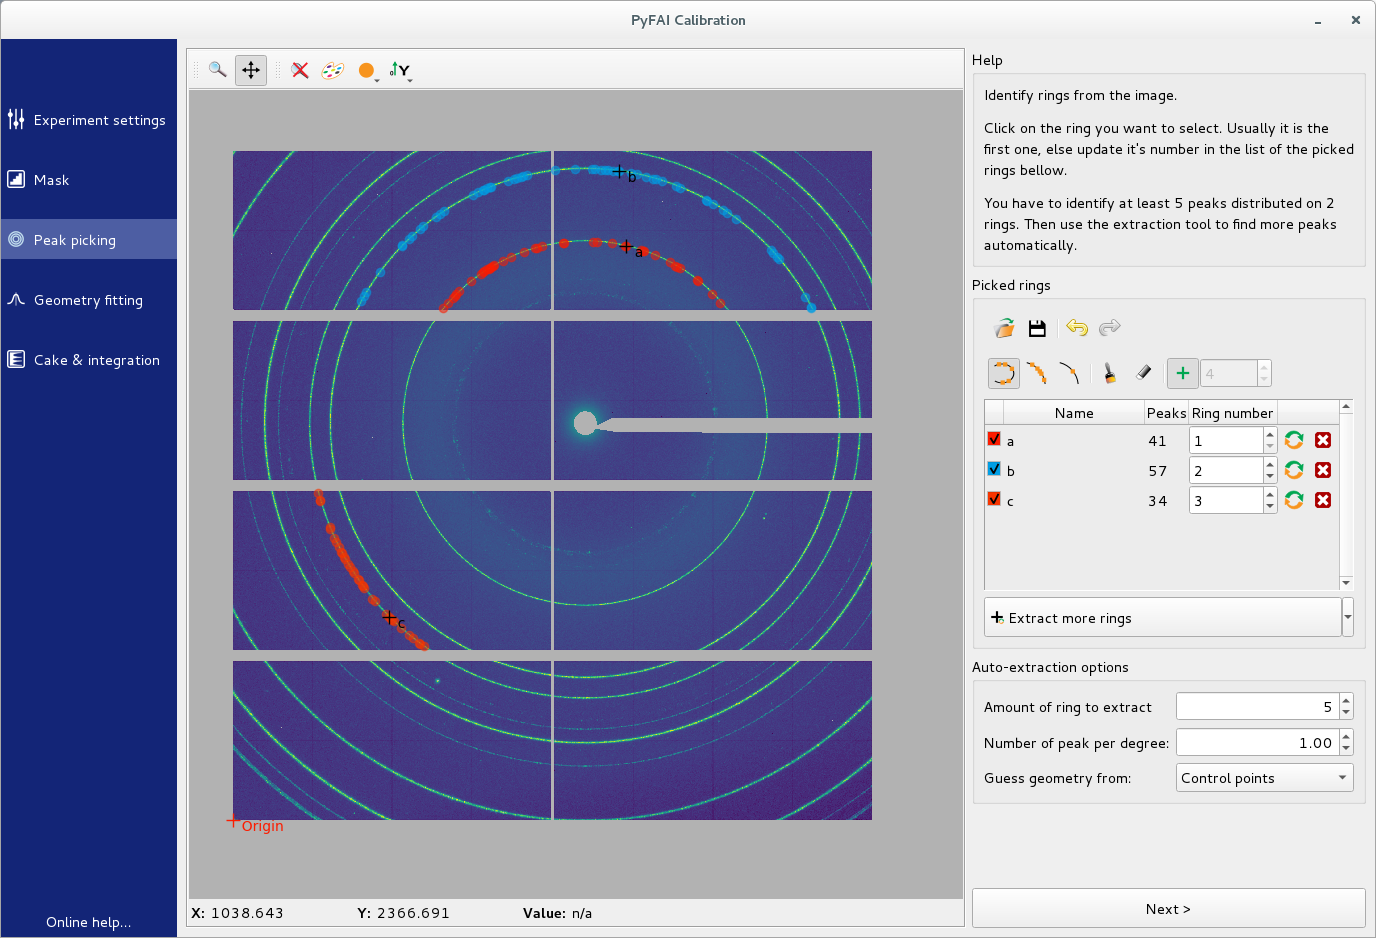
\includegraphics[width=15cm]{images/3_picking}
\caption{The peak-picking tool automatically selects groups of points close to the clicked peaks which then need to be assigned the proper ring number.}
\end{center}
\end{figure}
\begin{figure}
\label{calib_4}
\begin{center}
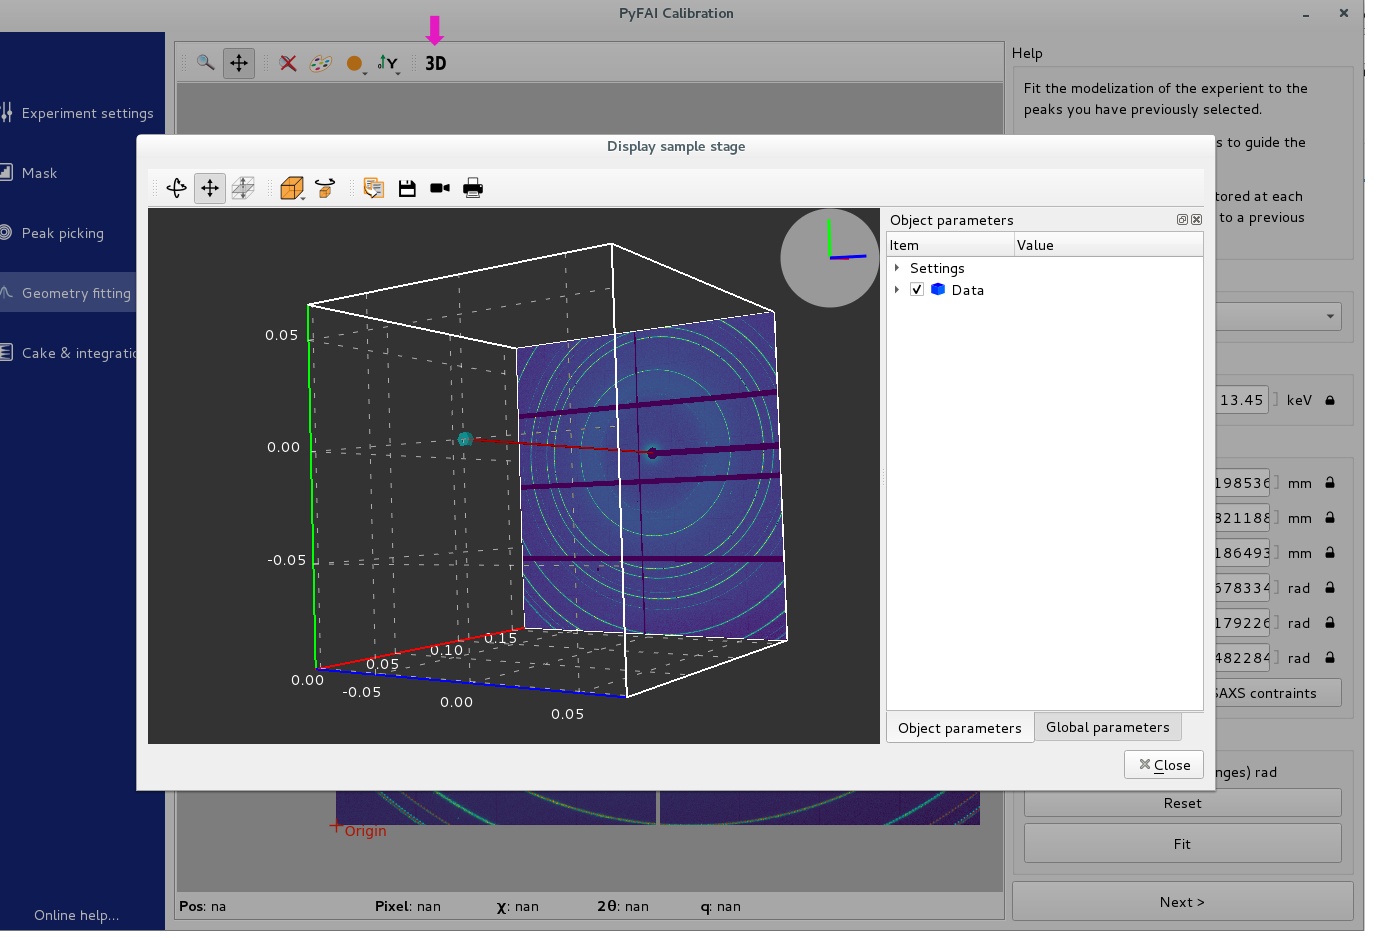
\includegraphics[width=15cm]{images/4_3d_view}
\caption{In the geometry fitting tab, each variable can be fixed, or left free for refinement within a given range. 
A 3D respresentation of the experimental setup allows visualizing the relative position of the sample, the direct beam and the detector after fitting.}
\end{center}
\end{figure}
\begin{figure}
\label{calib_5}
\begin{center}
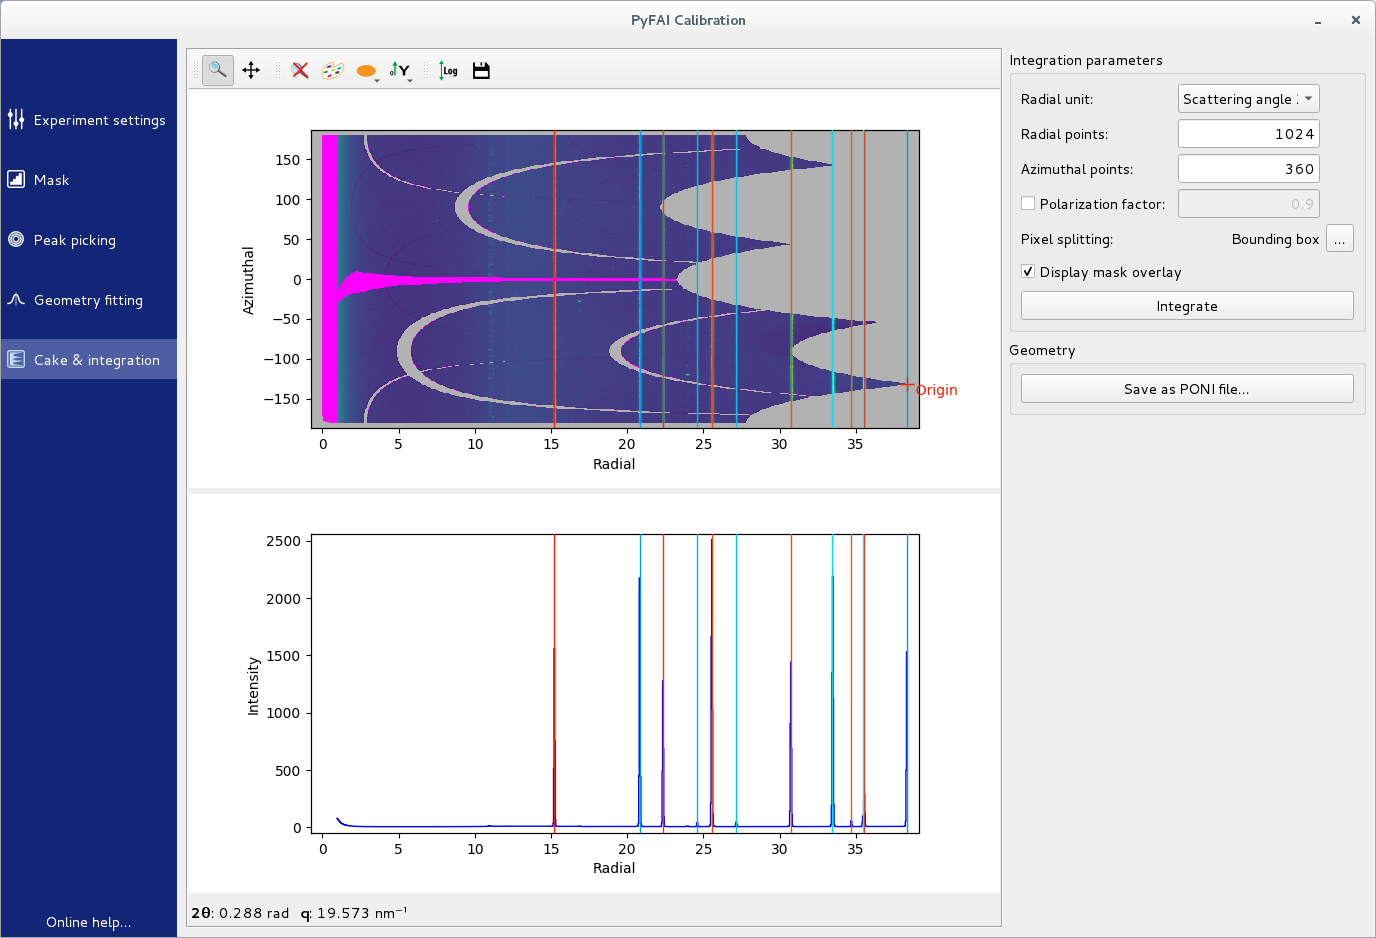
\includegraphics[width=15cm]{images/5_cake}
\caption{The cake and integration tab displays the 1D and 2D integrated image with the ring position overlaid to validate the quality of the calibration.}
\end{center}
\end{figure}

This new graphical user interface is now available with the
\textit{pyFAI-calib2} command and accounts for a simpler manual peak picking,
performes automatic ring extraction, geometry fitting and exports 
the regrouped data and the geometry. 
The online documentation of pyFAI contains a quick tutorial \cite{doc_gui}
designed for novice users to provide them their geometry in a couple of minutes.  
All graphical interfaces in pyFAI take advantage of the masking tools and HDF5
browsing widgets developed in the frame of the \textit{silx}
project \cite{silx_v0.5.0}, which streamlines the development effort around data
analysis. 
Diffraction image can be provided in HDF5 format \cite{collette_python_hdf5_2014}
or any of the dozens of fileformats supported by the FabIO library \cite{fabio}.

\section{Calibration of a detector on a moving stage}

The calibration of a detector mounted on a translation stage along the direct beam 
has successfully been exploited by Dawn \cite{Filik:vg5068} and GSAS-II \cite{Horn:co5127} 
to remove the correlation between the detector-distance and the energy of the beam. 
While those two software packages offer an intuitive user interface for those experiments, 
the modelisation of the translation stage remains hard-coded.
This section describes how to describe programatically a moving stage in pyFAI, 
calibrate the proposed model and use it to perform the azimuthal integration with many images. 

The calibration of the detector position on a fixed goniometer position can be
performed with pyFAI as long as several rings of the chosen calibrant are
present in the image and that five control points can be extracted from one
ring and at least one point from the second ring. 
Of course, more points provide a better fit but this limit may be an issue
if very small area detectors are used (i.e. the ImXPAD S10 is
as small as 80x120 pixels).

\subsection{Transformation of geometry}

Here, the difficulty is not in the calibration, but rather in the
variety of goniometers and translation stages which may be controlled by one or 
multiple motors.
%These motors are usually coupled with encoders, such as the actual position of
%the motors is known precisely.
The goniometer description implemented in pyFAI accepts an
arbitrary number of motors attached to the goniometer/translation stage. 
% which may be named (must be named for more than one moving motor). 
Let $motors = (motor_1, motor_2, \ldots, motor_n)$ be such motors. 

Calibrating the goniometer consists in:
\begin{itemize}
  \item defining a set of parameters for the goniometer, of arbitrary size:
  $params = param_1, param_2, \ldots, param_m$),
  \item defining a \textit{transformation function} $\Re$ which transforms motor positions
  and goniometer parameters into the six \textsc{poni}-parameters used by
  pyFAI,
  \item optimizing the parameter set of the goniometer (\textit{params}) so that
  for any position of the motors, the detector position can be expressed as
  a \textsc{poni}-parameters set.
\end{itemize}

This \textit{transformation function} takes hence motor names, and model-parameter names 
with their associated values (obtained after fitting), and returns
the six individual parameters used in \textit{pyFAI} to initialize an $AzimuthalIntegrator$; it can be formally
expressed as:

\begin{equation}
P_{pyFAI} = (dist, poni_1, poni_2, rot_1, rot_2, rot_3) = \Re_{params}(motors)
\end{equation}


The six \textsc{poni}-parameters returned 
%contained in the \textsc{poni}-file 
are then used to
calculate the $2\theta_{exp}$ position of the peaks over all control
points.
Those $2\theta_{exp}$ are compared to
the expected $2\theta_{theo}$ values calculated from the calibrant d-spacing and
the wavelength.

$$
\Delta 2\theta = 2\theta _{exp} - 2\theta _{theo} =
\arctan(\frac{r(P_{pyFAI})}{d(P_{pyFAI})}) -  2 \cdot
\arcsin(\frac{\lambda}{2d})
$$


The average of the squares of these differences is used as a cost function
to optimise those parameters using the \textit{scipy.optimize.minimize}
function from SciPy \cite{scipy}.

$$
CostFunct = \frac{ \sum\limits_{i \in CtlPts} {(\Delta 2\theta_i)^2}}
{count(CtlPts)} $$

From a computer engineering perspective, this \textit{transformation function}
should also be serializable to disk (e.g. in \textsc{json}-format) to allow
its restoration from a file without having to re-perform the calibration. 
To address this constraint, the \textit{NumExpr} library \cite{numexpr} is
used, enabling the user to provide textual mathematical formulae with
an arbitrary number of parameters (or $dof$) for the goniometer and as many parameters
as needed.

The definition of this function is simply the creation of an object from the 
\textit{pyFAI.goniometer.GeometryTransformation} class ($instantiation$), with a list of
motor names, parameter names as well as a set of six formulae, one for each of
the \textsc{poni}-parameters.
This will be explained in more detail by the following few examples.

\subsection{A simple example: the translation table}

At the  ESRF, the protein crystallography beam-lines use large pixel detectors
(typically Pilatus 6M from Dectris) placed on a translation stage which allows
collecting the data at the optimal distance: shorter sample-to-detector
distances to explore the region for high-$q$ 
or longer distances for better Bragg peak separation. 

The \textit{MX-calibrate} tool from the pyFAI suite is available for
calibrating many images taken at various distances.
This can also be interpreted in terms of a goniometer setup (actually a translation table) where the sample-to-detector distance is modelled as a
simple linear function of the translation table position:

\begin{verbatim}
from pyFAI.goniometer import GeometryTransformation
gt = GeometryTransformation(param_names = ["dist_offset", "dist_scale", 
                                        "poni1", "poni2", "rot1", "rot2"],
                            pos_names = ["position"],
                            dist_expr="position * dist_scale + dist_offset", 
                            poni1_expr="poni1",
                            poni2_expr="poni2", 
                            rot1_expr="rot1", 
                            rot2_expr="rot2", 
                            rot3_expr="0.0")
\end{verbatim}
 
In the example above, we chose to use six parameters for the goniometer
geometry, most of them being exactly the same as those of pyFAI: 
$poni_1$, $poni_2$, $rot_1$
and $rot_2$. 
$rot_3$ is forced to zero while the distance is defined as a 
linear function of the motor position. 
This actually makes six $dof$ to be refined.
Motor names should be declared as a list and assigned to \textit{pos names}. 
If no motor names are provided, a single motor  configuration (called $pos$)
is assumed.

The content of this tutorial is available as a Jupyter
notebook \cite{ipython} and part of the official documentation of pyFAI:
\cite{translation_table}, this document is directly visible in a web-browser. 
In addition, one can replay the notebook with Jupyter and the notebook is
self-consistent: all images are automatically downloaded and cells can be
modified or adapted.
The notebook presents the usage of the \textit{transformation function} class
together with the translation table refinement.
Initially, this set of data was calibrated using the ``MX-calibrate'' tool
that automatically extracts the control points from images taken at
ESRF ID29 beam-lines (Protein crystallography beam-line, energy: 12.75 keV) from
the metadata written in the image headers, thus a set of control points is
available prior to processing the data. 
The translation table is calibrated using all control points
and this \textit{transformation function}.
As a result, all images have been integrated azimuthally.
The Figure \ref{id29} is a zoom on the two first Bragg peaks of CeO$_2$. 
The blue curve corresponds to this initial model refined; the two peaks look
``doubled'' indicating a poor modelling of the geometry.

\begin{figure}
\label{id29}
\begin{center}
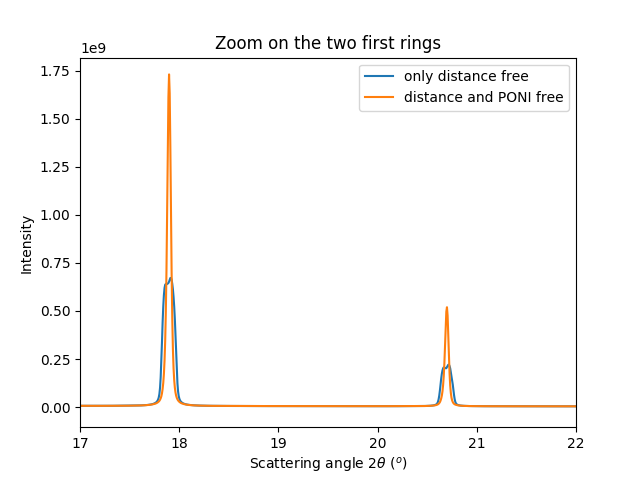
\includegraphics[width=9cm]{images/TranslationTable}
\caption{Powder diffraction profile obtained from seven images acquired
at various distances from 15 to 45 centimeters. 
The translation table position is combined with 6 (resp. 8) parameters model
fitted where the $dist$ (resp. $dist$, $poni_1$ and $poni_2$) depends on the
table position.}
\end{center}
\end{figure}

To address this poor modelling, another \textit{transformation function} is
defined, with a few additional $dof$ on the \textsc{poni} position
(i.e. the translation table is not perfectly parallel to the incident beam).
%(linear dependency of the \textsc{poni} with the table position).
Once the three parameters ($dist$, $poni_1$ and $poni_2$) have been re-fitted and 
all data integrated with the new model, one obtains the orange
curve in Figure \ref{id29}. 
Its peaks are much sharper than previously and the residual cost is
about five times smaller, indicating a much better fit.

This example shows that the \textsc{poni} is moving on the detector
plane by 1 \textperthousand horizontally and 
4 \textperthousand vertically.
This ``large'' vertical deviation has been confirmed by the beam-line staff and
is related to the last focusing mirror placed just before the sample, causing the
beam to dive.
Once everything is fitted, the quality of the geometry obtained is perfectly
suited to powder diffraction experiments for any detector position.
  
\subsection{A more realistic example: a single axis goniometer}

Probably the main application of this work is to place a small size detector
on a goniometer $2\theta$ arm. 

When the detector arm is moving vertically, a simple \textit{geometry
transformation} is defined with $rot_2$ (in radians) as a
linear transformation of the motor position, $pos$, (measured in degrees).
The scale parameter, $scale = \pi / 180$, is used to convert degrees to radians.
The other parameters $dist$, $poni_1$, $poni_2$ and $rot_1$ are directly mapped
to pyFAI's parameters.
As previously, $rot_3$ is kept fixed at zero.

\begin{verbatim}
from pyFAI.goniometer import GeometryTransformation
goniotrans = GeometryTransformation(param_names = ["dist", "poni1", "poni2", "rot1",
                                                   "rot2_offset", "rot2_scale"],
                                    dist_expr="dist", 
                                    poni1_expr="poni1",
                                    poni2_expr="poni2", 
                                    rot1_expr="rot1", 
                                    rot2_expr="rot2_scale * pos + rot2_offset", 
                                    rot3_expr="0.0")
\end{verbatim}


This example is also available in a Jupyter notebook \cite{rotation_pilatus} 
and the workflow used is depicted in Figure \ref{workflow}.
This experiment has been performed using a single module (100k) Pilatus
detector which is mounted on a vertically moving $2\theta$ arm, varying 
from 5 to 65 degrees in half-degree steps on the ROBL beam-line
\cite{Kvashnina:vv5126}, ESRF BM20.
In this experiment, 121 diffraction images of LaB$_6$
reference compound material were acquired.
Due to the small size of the detector (487x197 pixels),
some of the images present no ring at all (especially at low $2\theta$ angle),
most have one ring and only a few images display 2 rings.

\begin{figure}
\label{workflow}
\begin{center}

\includegraphics[width=9cm]{images/workflow}
\caption{Workflow used to calibrate the set of 121 Pilatus 100k images on a
moving $2\theta$ arm and detailed in the \textit{Jupyter Notebook} given in  
\cite{rotation_pilatus}.}
\end{center}
\end{figure}

The first images presenting two rings correspond to goniometer positions above
30 degrees. 
Four images, taken at goniometer angles of 31.5, 33 and 35 and 35.5
degrees have been manually calibrated using the \textit{pyFAI-calib2} tool
presented in the previous section.
This manual calibration is rather tedious and unstable due to the small
curvature of the rings on the detector image. 
The rotation along axis 1 of the detector ($rot_1=0$) has been kept fixed to
guarantee some consistency between the four images.

An initial simple model with a set of parameters where $rot_2$ is equal to the
goniometer angle has first led to convergence with some constraints and
bounds.
In a second step, twenty images in the neighbourhood of the first ones have been
added to the model, their peaks extracted according to the initial model and the
model refined using the control points from the twenty images.
Then, all other images have been added to the model, and additional control
points have been automatically extracted from all images according to the
previous geometry model.
After all constraints and bounds have been removed, the model has been refined
again and used to generate a \textit{MultiGeometry} object, able to integrate many
images together.
After integration of all 121 images, the powder diffraction pattern displayed
in Figure \ref{bm20}, orange curve, is obtained.
All peaks of the curve appear at the correct scattering angle but
the first ones looks exceedingly broad. 

\begin{figure}
\label{bm20}
\begin{center}
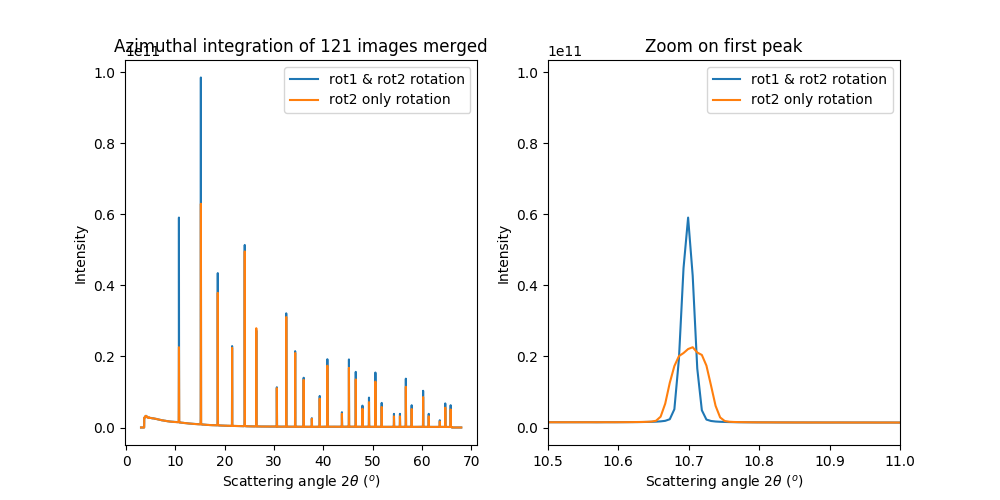
\includegraphics[width=9cm]{images/gonio}
\caption{Powder diffraction pattern obtained from 121 images acquired
at goniometer angles ranging from 5 to 65 degrees. On the right-hand site,
a close-up view on the first peak following a simple model (6 $dof$,
 in orange) or according a model where two parameters are
functions of the goniometer position (7 $dof$, in blue).}
\end{center}
\end{figure}


This broadening is confirmed by looking at the first ring's image, where the
goniometer angle was set to 10 degrees (Figure \ref{bm20_10}).
The expected position of the ring (dashed red line) does not correspond
properly to the actual ring (yellow on the image). The extracted control points 
are plotted in blue.

\begin{figure}
\label{bm20_10}
\begin{center}
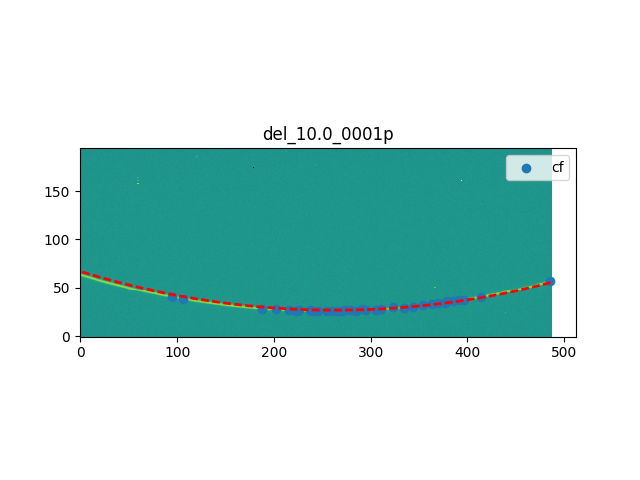
\includegraphics[width=9cm]{images/gonio_10}
\caption{Diffraction image taken with the goniometer arm at 10 degrees.
The control points are in blue and the expected ring of the simple model
($rot2=f(pos)$) is the dashed red line. This highlights the need for $rot_1$
to depend on the goniometer position.}
\end{center}
\end{figure}

Another model was tested, allowing also the $rot_1$ value to scale with the 
goniometer position. 
After refinement, the cost function dropped by a factor two and
the low angle peaks became sharp (blue curve in Figure \ref{bm20}). 

This parameter set was saved and allowed a few other compounds to be analysed and
compared to the same pattern recorded via a moving point detector. 
The signal/noise ratio was found to be better with an acquisition time which was one order
of magnitude shorter than previously, thus opening new prospects for
the ROBL beam-line.

A third example of goniometer calibration is available in \cite{rotation_xpad}. 
It corresponds to the calibration of an ImXPAD detector \cite{BOUDET200341}
composed of 8 stripes of 7 modules, many of which are defective.
This detector is mounted on the goniometer arm at the D2AM beam-line
\cite{Ferrer:ri0008}, ESRF BM02. 
This example is conceptually the same as the the one from the ROBL beam-line,
with a few differences:
\begin{itemize}
  \item all images are fitted directly with 8 $dof$,
  \item the detector being larger, the calculation time is
        longer, especially when it comes to ring extraction,
  \item the mask needs some extra care to remove a few hot pixels,
  \item the detector is mounted rotated by 90 degrees on the arm, thus $rot_3=\pi/2$.
\end{itemize}

This generic method has even been extended to strip detectors 
like the Mythen detector manufactured by Dectris as shown in the tutorial on the 
calibration of the array of 9 Mythen detectors \cite{rotation_mythen}, mounted on 
the goniometer arm of beam-line Cristal at Synchrotron Soleil.  

\section{Outlook}

The goniometer description in this work can be adapted to
many types of goniometer.
The \textit{TransformationFunction} class presented in the notebook may be extended
in the future to use \textit{libhkl} \cite{libhkl} which contains already many
diffractometer geometries with their associated rotation matrices. 

Different generations of pixel detectors have seen their pixel sizes
shrinking:
from $172 \mu m$ for the Pilatus, $130 \mu m$ for ImXPAD, $75 \mu m$ for the
Eiger and $55 \mu m$ for Medipix-based chips \ldots, and probably even less for
future generation detectors.
As the resolution of the powder diffraction diagram obtained is limited by the
pixel size (and the sample-detector distance), this shrinkage of
pixel sizes leads naturally to higher quality powder
diffraction patterns.
Unfortunately, to keep the surface of the detector constant, one would need
to multiply the number of pixels by the square of the pixel size reduction
factor, and the associated infrastructure for read-out and data transfer
accordingly.
Moving the detector offers a flexibility which partially removes this
limitation.

\section{Conclusion}

The new graphical user interface of pyFAI has been developed to ease the
calibration of an experimental setup with static detector, especially for
novice users.
The concept of calibration of the detector position has been extended to fit
the detector position with the motion of a goniometer.   
Once a few fixed positions of the goniometer have been calibrated, a model can
be optimized to determine the detector position at any goniometer
configuration.
By acquiring multiple images at various positions, these images can be
integrated together to produce a high-$q$ powder diffraction pattern of
quality equivalent to the one acquired with a much larger detector. 
 
\ack{Acknowledgements}

We would like to thank all ESRF beam-line teams for supporting the
pyFAI development, and especially David Flot from the MX-group who provided the
data of the translation table and Nils Blanc and Christoph Hennig from the the
beam-lines BM02 (D2AM) and BM20 (ROBL) (respectively) for the goniometer data. 
They gracefully provided beam time and test data to allow debugging this 
goniometer optimisation tool.
We would also like to thank the French CNRS for financing the IR-DRX project
in 2015 and 2016, which acted as a catalyst on the goniometer refinement,
and the other participants in the project, especially Serge Cohen from the
Ipanema institute, the DiffAbs and Cristal beam-lines and Frédéric-Emmanuel Picca 
from Synchrotron Soleil.
In the instrumentation services and development division (ISDD) of the ESRF  we
would like to thank V. Armando Solé, head of the data analysis unit and leader of 
the \textit{silx} project, and all our colleagues from the \textit{silx}
project:
Thomas Vincent, Henri Payno, Damien Naudet and  Pierre Knobel for their support and ideas. 
A great thank you to Carsten Detlefs for his contribution to the documentation of the geometry in pyFAI. 
Finally we would like to dedicate this article to our colleague and friend Claudio Ferrero, who suddenly passed away in 2018. 

\bibliographystyle{iucr}
\bibliography{biblio}


\end{document}
